% Chapter Template

\chapter{Discussion} % Main chapter title

\label{Chapter6} % Change X to a consecutive number; for referencing this chapter elsewhere, use \ref{ChapterX}

\lhead{Chapter 6. \emph{Discussion}} % Change X to a consecutive number; this is for the header on each page - perhaps a shortened title

%----------------------------------------------------------------------------------------
%	SECTION 1
%----------------------------------------------------------------------------------------
\section{Discussion}

We have analysed the EEG signals from 64 channels to detect the mind wandering state using some basic machine learning techniques.After trying 6 machine learning classifiers, we are able to detect MW and Alertness state with 87\% accuracy.By analysing the test results from all six classifiers, we observed a pattern that is the precision and recall of  Alertness state detection is higher than  Mind Wandering state.So, we can say that we are able to predict Alertness more precisely than MW.And similarly you can see  that F1-score for MW is lower than Alertness (Figure \ref{fig:test_score}).And you can also see different comparison in the Figure \ref{fig:test_score}.


\begin{figure}
    \subfigure[]{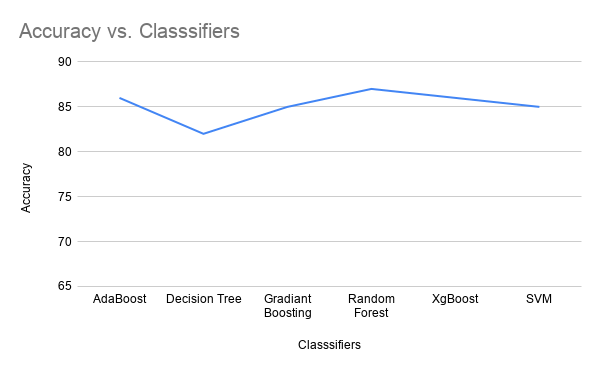
\includegraphics[width=0.49\textwidth]{Pictures/Accuracy vs. Classsifiers (1).png}}
    \subfigure[]{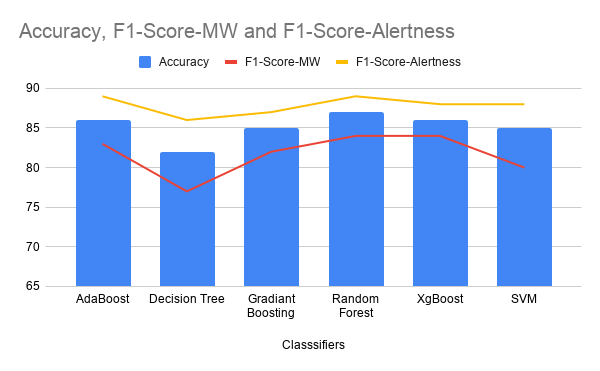
\includegraphics[width=0.49\textwidth]{Pictures/Accuracy, F1-Score-MW and F1-Score-Alertness.png}}
    \subfigure[]{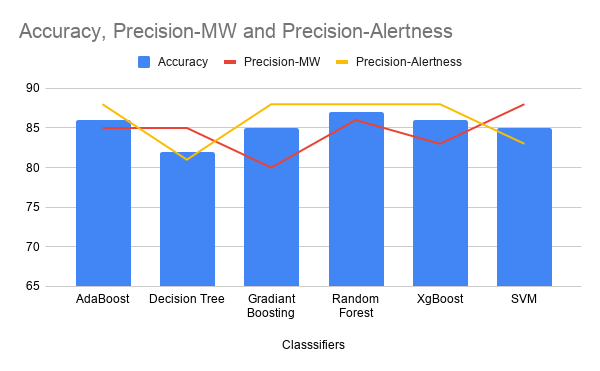
\includegraphics[width=0.49\textwidth]{Pictures/Accuracy, Precision-MW and Precision-Alertness.png}}
    \subfigure[]{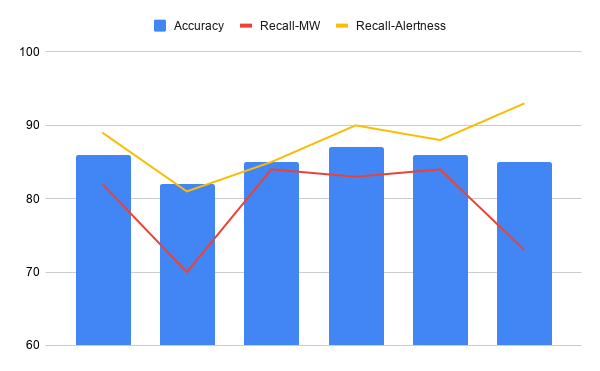
\includegraphics[width=0.49\textwidth]{Pictures/chart (1).png}}
    
    \subfigure[]{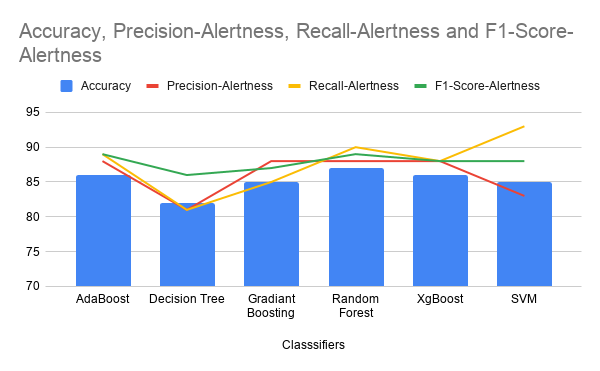
\includegraphics[width=0.49\textwidth]{Pictures/Accuracy, Precision-Alertness, Recall-Alertness and F1-Score-Alertness (1).png}}
    \subfigure[]{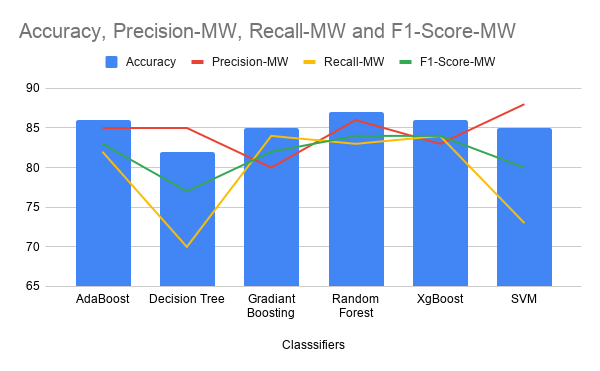
\includegraphics[width=0.49\textwidth]{Pictures/Accuracy, Precision-MW, Recall-MW and F1-Score-MW.png}}
    \centering
    % 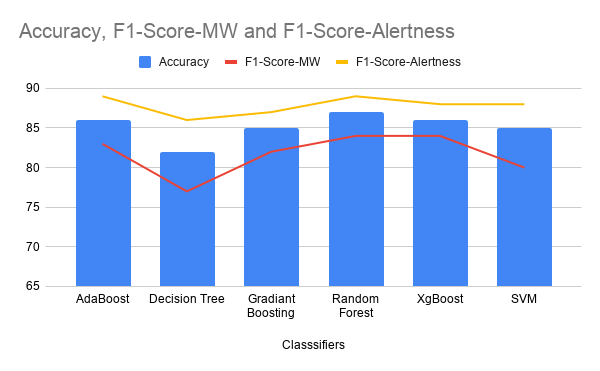
\includegraphics[width=10cm]{Pictures/Accuracy, F1-Score-MW and F1-Score-Alertness.png}
    \caption{Classifier results,bar chart is for accuracy and line chart is for precision,recall and F1-score (a) accuracy vs classifier, (b) comparison of F1-score , (c) comparison of precision, and (d) comparison of recall  for MW and Alertness for different classifier,  (e) comparison of precision,recall and f1-score for alertness for different classifier, and (f)  comparison of precision,recall and f1-score for MW for different classifier,  }
    \label{fig:test_score}
\end{figure}


The highest accuracy, that we got by analysing EEG-signals from 64 channels using 6 different basic machine learning  classifiers is 87\% which is higher than any research have been done in this area.We have got the highest accuracy on Random Forest classifier.Before applying classifier we extracted MW \& alertness data from continuous channel signals, normalized them,extracted feature set for all 64 channels of size 52 and flattened them by concatenating each channel data.Then we have applied classifiers.By comparing all the results we can safely deduce that by using XgBoost,Random Forest and Ada-Boost ML classifiers to detect MW and alertness state with a 86-87 \% accuracy.